\documentclass{article}
\usepackage[utf8]{inputenc}
\usepackage[margin=1.0in]{geometry}
\usepackage{graphicx}
\usepackage{caption}
\usepackage{subcaption}
\usepackage{wrapfig}
\usepackage{amsmath}
\usepackage{caption}
\let\vec\mathbf

\title{Image Stitching}
\author{Neal Bayya and Alexey Didenkov}
\date{April 3, 2019}

\DeclareMathOperator{\taninv}{tan^{-1}}

\begin{document}

\maketitle

\section{Introduction}
Stitching images is one of the oldest and widely-used applications of computer vision.
The demand for image stitching originates from the photogrammetry and film photography communities, where it was used to ease methods for manually  computing distances and eliminate the need for expensive wide-angle cameras.
While these earlier approaches relied on rigorous technology such as \textit{ground-control points} or special \textit{rotating cameras}, advancements on the computer vision side of things made these methods more convenient with time.
Modern image stitching algorithms are presently used for combining satellite imagery and creating panoramas on digital cameras.
Today, we will discus how to represent, align, and then combine similarities between images.


\section{Motion Models}
Image stitching fundamentally relies on finding and relating similarities between images.
With that in mind, we need to have a good way to describe these relations in order to find them in the first place.
Specifically, we must find a mathematical model that relates pixel coordinates of one image to that of another.

\subsection{Planar Perspective}
The simplest approach to aligning images is with 2D rotation and translation.
This works fine for small motions such as when stabilizing videos, but otherwise creates visible seams.
We can do better.

Recall that each camera has intrinsic parameters that can be arranged in a $3\times 3$ matrix $\vec{K}$.
Combined with extrinsic 3D rotation and translation parameters, we can form a $3\times 4$ \textit{projection matrix} that maps homogeneous 3D world coordinates to screen coordinates:
$$
\vec{P}=\vec{K}[\boldsymbol{R} | \vec{t}],\quad
\vec{K}= \left[ \begin{array}{lll}{\mathrm{f}_{\mathrm{x}}} & {0} & {\mathrm{c}_{\mathrm{x}}} \\ {0} & {\mathrm{f}_{\mathrm{y}}} & {\mathrm{c}_{y}} \\ {0} & {0} & {1}\end{array}\right]
$$
If we extend this $\vec{P}$ matrix to a $4\times 4$ $\tilde{\vec{P}}$, we can invert it and perform the reverse operation.
Then, mapping a pixel in one image to 3D coordinates and then to another image becomes:
$$ 
\tilde{\boldsymbol{x}}_{1} \sim \tilde{\boldsymbol{P}}_{1} \tilde{\boldsymbol{P}}_{0}^{-1} \tilde{\boldsymbol{x}}_{0}=\boldsymbol{M}_{10} \tilde{\boldsymbol{x}}_{0}
$$
\begin{wrapfigure}{r}{0.225\textwidth}
  \vspace{-40pt}
  \begin{center}
    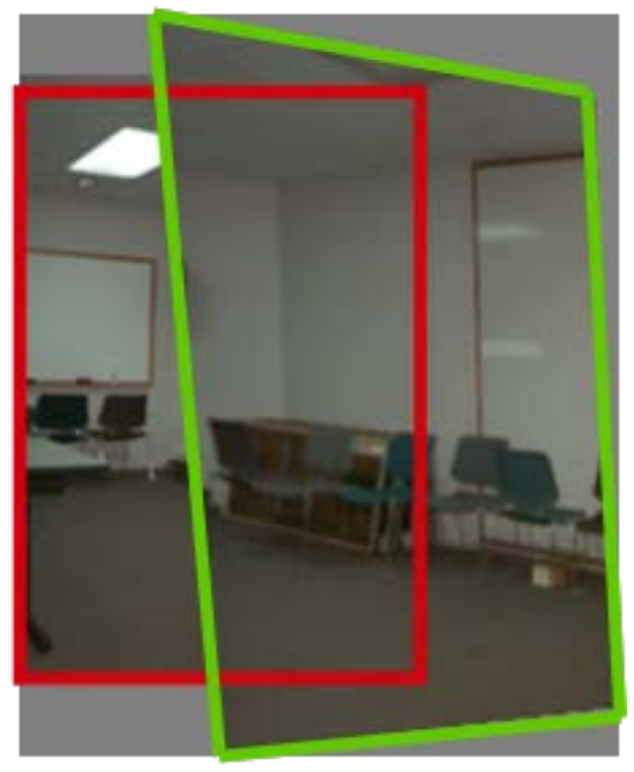
\includegraphics[width=0.225\textwidth]{perspective.png}
  \end{center}
  \vspace{-20pt}
  \caption{Perspective Transform}
  \vspace{-30pt}
\end{wrapfigure}
In the condition that the real-world points \textbf{all lie on a plane}, we can ignore the last row and column of the $4\times 4$ matrix $\boldsymbol{M}_{10}$, reducing it to a $3\times 3$ $\tilde{\boldsymbol{H}}_{10}$:
$$ 
\tilde{\boldsymbol{x}}_{1} \sim \tilde{\boldsymbol{H}}_{10} \tilde{\boldsymbol{x}}_{0}
$$
This looks awfully familiar to the 2D \textbf{perspective transform} as covered in the transformation lecture:
$$ 
k \left[ \begin{array}{l}{x^{\prime}} \\ {y^{\prime}} \\ {1}\end{array}\right]=\left[ \begin{array}{lll}{h_{00}} & {h_{01}} & {h_{02}} \\ {h_{10}} & {h_{11}} & {h_{12}} \\ {h_{20}} & {h_{21}} & {h_{22}}\end{array}\right] \left[ \begin{array}{l}{x} \\ {y} \\ {1}\end{array}\right]
$$
Although this transformation has 9 parameters, it is invariant to scale — an extra parameter $k$ is discarded afterwards.
Thus, the matrix has 8 degrees of freedom — the $x$- and $y$-coordinates of each of the four corners.

The actual $h$-parameters are found by solving the least squares fitting problem through robust methods such as RANSAC.
Though this has been done on raw pixel values in the past, modern approaches typically find transformations based on pairing up \textit{feature descriptors}, such as SIFT points.

Although the assumption that all points lie on a plane makes this model non-versatile, it can be used in situations such as when taking \textbf{pictures of a whiteboard} from multiple positions and angles.

\subsection{Rotational}
Often, such as when taking \textbf{panoramas}, the camera stays in the same location while only rotating.
This is equivalent to assuming that all points are infinitely far away from the camera, i.e. lying on the \textit{plane at infinity}.
This invites us to use the reduced $\tilde{\boldsymbol{H}}_{10}$ matrix from the previous section, the upper-left $3\times 3$ sub-matrix of
$$
\boldsymbol{M}_{10} = \tilde{\boldsymbol{P}}_{1} \tilde{\boldsymbol{P}}_{0}^{-1}
$$
Since the camera does not move laterally, the extrinsic translation parameters are all zeroes.
This reduces the projective matrix to $\vec{P}=\vec{K}\vec{R}$ and lets us write out $\tilde{\boldsymbol{H}}_{10}$ only using $3\times 3$ matrices:
$$ 
\tilde{\boldsymbol{H}}_{10}=\boldsymbol{K}_{1} \boldsymbol{R}_{1} \boldsymbol{R}_{0}^{-1} \boldsymbol{K}_{0}^{-1}=\boldsymbol{K}_{1} \boldsymbol{R}_{10} \boldsymbol{K}_{0}^{-1}
$$
\begin{wrapfigure}{r}{0.25\textwidth}
  \vspace{-30pt}
  \begin{center}
    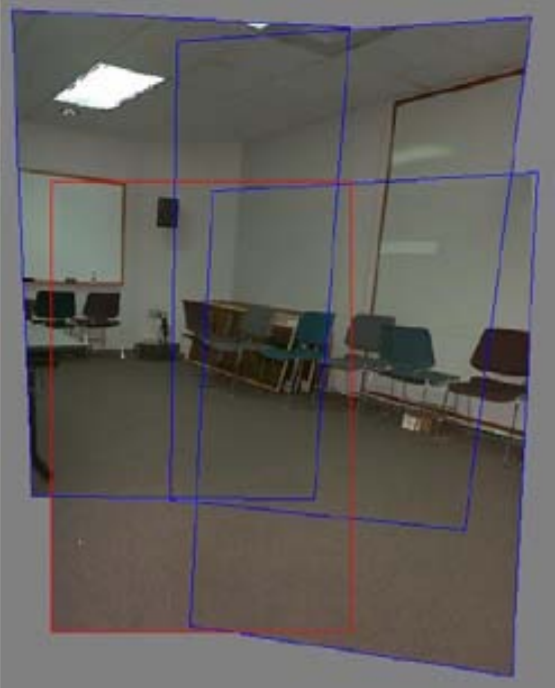
\includegraphics[width=0.25\textwidth]{rotation.png}
  \end{center}
  \vspace{-15pt}
  \caption{Rotation Model}
  \vspace{-30pt}
\end{wrapfigure}
Assuming that $c_x=c_y=0$ (pixel indexing starts from the optical center), $\vec{K}$ and $\vec{K^-1}$ become diagonal matrices.
Further assuming that $f_x = f_y = f$ reduces the equation to
$$ 
\left[ \begin{array}{l}{x_{1}} \\ {y_{1}} \\ {f_{1}}\end{array}\right] \sim \boldsymbol{R}_{10} \left[ \begin{array}{l}{x_{0}} \\ {y_{0}} \\ {f_{0}}\end{array}\right],\quad
\boldsymbol{R}_{10} = \boldsymbol{R}_{1} \boldsymbol{R}_{0}^{-1}
$$
If the focal length is constant or known, the tuning process becomes more stable as it no longer needs to find intrinsic parameters.
This has the effect of reducing the degrees of freedom we have to fit on \textbf{down to 3}.
In practice, tuning can be made even easier by using the small-angle approximation and finding step-wise perturbations instead.

\subsubsection{Cylindrical Coordinates} 
Rather than depending on the motion models that we have seen insofar which have high degrees of freedom, we can warp the images in a cylindrical coordinate system and restrict our motion of alignment to translation. 
However, this will only work with a level camera or a known tilt angle. As you can see from Figure \ref{cylinder}, the 3D cylindrical coordinates $\left( \sin\theta, h, \cos\theta\right)$ correspond to $\left( x,y,f \right)$. \\
\begin{wrapfigure}{r}{0.325\textwidth}
  \vspace{-45pt}
  \begin{center}
    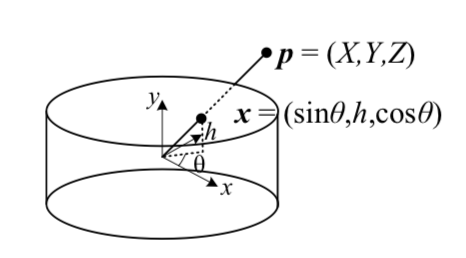
\includegraphics[width=0.3\textwidth]{cylindrical.png}
  \end{center}
  \caption{Cylindrical Warp}
  \label{cylinder}
  \vspace{-35pt}
\end{wrapfigure}

From this correspondence, \textit{Szeliski and Shum 1997} derived the formula for the warped coordinates to be:
\begin{eqnarray*}
x' &= s\theta &= s\taninv \frac{x}{f} \\
y' &= sh &= s\frac{y}{\sqrt{x^2 + f^2}}
\end{eqnarray*}
where s can be thought of as the radius of the cylinder.
The selection of s actually dictates the resolution of the stitched output panorama resolution, and it is commonly set to $f$. The inverse mapping is given by 
\begin{eqnarray*}
x &= f\tan\theta &= f\tan \frac{x'}{s}  \\
y &= h\sqrt{x^2 + f^2} &= f\frac{y'}{s}\sec{x'}{s} 
\end{eqnarray*}

\subsubsection{Spherical Coordinates}
Images may also be projected in spherical coordinates if the camera motion includes a full sphere of of views.
Figure \ref{sphere} demonstrates that the spherical coordinates $\left( \sin\theta\cos\phi, \sin\phi, \cos\theta\cos\phi\right)$ corresponds to $\left( x, y, f \right)$.
The correspondence given by \textit{Szeliski and Shum 1997} is
\begin{eqnarray*}
x' &=& s\taninv\frac{x}{f}  \\
y' &=& s\taninv \frac{y}{\sqrt{x^2 + f^2}}
\end{eqnarray*}

\begin{wrapfigure}{r}{0.375\textwidth}
  \vspace{-90pt}
  \begin{center}
    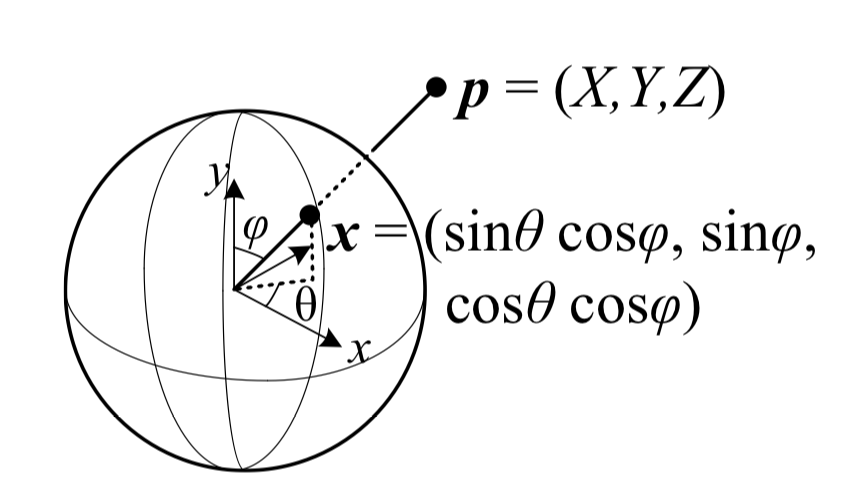
\includegraphics[width=0.35\textwidth]{sphere.png}
  \end{center}
  \caption{Spherical Warp}
  \label{sphere}
  \vspace{-50pt}
\end{wrapfigure}
where $s$ may again be thought of as the radius of the sphere. 
The inverse relationship is as follows:
\begin{eqnarray*}
x &=& f\tan\frac{x'}{s} \\
y &=& f\tan\frac{y'}{s}\sec\frac{x'}{s}
\end{eqnarray*}
In practice, spherical coordinates are used in image stitching when your camera is free to rotate around its vertical axis.
Under the spherical coordinate system, images that are rotated at different angles are related with a simple translation (that is, when operating with $x'$ and $y'$).
Professional photographers often have camera systems which take images at specific intervals as the camera rotates around the vertical axis for precision.


\section{Stitching}
Our next task is to stitch the images together.
Having found a relation between the coordinate domains of the two images, how exactly do we combine them into a single domain?

\subsection{Composite Surface}
When deciding which domain to project the stitched image onto, a simple answer would be to choose one that already exists.
This means selecting a \textbf{reference} image and warping all the others around it in a \textbf{flat} panorama.

Now, imagine that you went outside and took some pictures of the night sky.
If you try to combine these images naïvely you will notice weird distortions that get worse the further you go from the reference image.
After all, the sky is a dome — attempting to flatten it out will severely stretch its edges.

Generally, this happens when the field of view exceeds about $90^\circ$. 
To fix this, one can project their panorama on a different composite surface, such as a \textbf{cylindrical}, \textbf{spherical}, or \textbf{cubic} map.

\subsection{Sampling Issues}
After putting pixel values through our mathematical models we get non-integer pixel locations.
This means that we need to find a way to discretize them without creating visual artifacts.
This can be done based on distance, or other methods such as higher-order (e.g. \textit{cubic}) interpolators, \textit{Gaussian averaging}, or \textit{MIP mapping}.
Also, a pre-filter is necessary to avoid aliasing in cases with resolution differences.

\subsection{Pixel Selection}
After placing all image points in a common transformation space, we end up with many overlapping areas and are tasked with combining information.
A simple approach would be to \textit{average} all images in areas of overlap, but this creates some problems:
\begin{itemize}
    \itemsep -0.15em
    \item Presence of bright objects in certain images but not others can cause \textit{exposure differences} — cameras typically darken the background for such images to compensate.
    Then, simple averaging will produce \textbf{seams} in places where such images have an edge.
    \item \textit{Moving objects} will become translucent in what is known as \textbf{ghosting}.
    \item Mis-registration due to various alignment errors will cause \textbf{blurring}.
\end{itemize}
More complex weighting methods have been developed to deal with these problems:
\begin{itemize}
    \itemsep -0.15em
    \item Ghosts can be removed by taking the \textit{median} instead.
    \item Seams at image edges can be blended by weighing pixels more if they are closer to their original image's center.
    This is called \textbf{feathering}.
    \begin{itemize}
        \itemsep -0.15em
        \item Raising distances to a higher power will make transitions sharper, much like in a \textit{p-norm}.
        This lets us vary the amount of blurring we do, providing a trade-off between solving misalignment and seams.
        \item It is favorable to blend more where images agree and less where they don't.
        Certain algorithms automatically vary the amount of blending based on how closely the overlapping regions align.
    \end{itemize}
    \item \textit{Minimum likelihood} can be used if retaining moving objects is desirable.
    \item A better quality blend can be achieved with \textit{Laplacian pyramid blending}.
\end{itemize}

\section{Global Alignment}
So far, we have focused mainly on combining pairs of images.
However, combinations typically use a large number of source images, and can be made better by taking them all into account before deciding how to stitch.

\subsection{Bundle Adjustment}
The simple solution is to keep adding images to the panorama in the order that they are given. As previously mentioned, in flat panoramas images will be distorted if the reference image is not chosen right.
In $360^\circ$ panoramas, accumulating errors can cause massive gaps or overlaps upon attempting to connect the ends.

The solution is to adjust alignment while minimizing errors for the collection as a whole, also called \textbf{bundle adjustment}.
This is similar to tuning transformation parameters for pairs of images, but now it is done for all images at once.

Further improvements can be made — frequent features can be prioritized less to avoid being overweighted, modifying the loss to compute against 3D point positions can speed up the process by making matrices sparse.

\subsection{Recognizing Panoramas}
Sometimes, people take pictures of the same scene without realizing that a panorama could be created.
In such cases, it would be useful to automatically detect panoramas from a collection of unsorted images, some of which may not belong in a panorama at all.

Similarly to bundle adjustment, overlaps between images are computed and minimized. The main difference is that edge connections can now be discarded if they exceed a certain threshold.
Needless to say, this threshold is a fine balance between false positives due to similar structures and false negatives due to moving objects.

\section{Other Errors}
As previously mentioned, errors in circular panoramas can accumulate and result in large gaps or overlaps.
Another solution to solving this is \textbf{gap closing}, an approach that relies on adjusting the focal length.
We can update the focal length based on the amount of misregistration between the rotation matrices of the first and last image according to the following rule: $f' = f\left(1-\theta_g/360\right)$.
While this correction formula only works with a camera rotating along one dimension, there are extensions for arbitrary camera motions.

Even then, we might still find that our images look blurry or ghosted due to varying errors. \textbf{Parallax removal} aims to solve this by applying warping transformations to misaligned regions.

\end{document}